Als je op de command line bent heb je een commandprompt. De commandprompt is het deel voor de cursor, zie \ref{fig:console}

\begin{figure}[h]
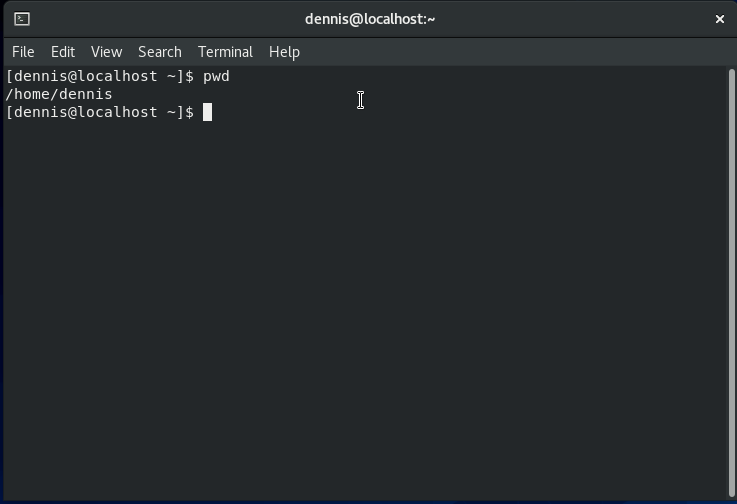
\includegraphics[width=0.8\linewidth]{linuxreader-img022.png}
	\label{fig:console}
	\caption{Console}
\end{figure}

Links staat de login naam, dennis, daarnaast op welke host je bent in gelogd, localhost, daarna volgt de directory
waarin je je nu bevindt, \~{}, en tot slot de prompt voor een normale gebruiker: \$. Als je ingelogt bent als root dan staat er inplaats van een \$ een \#. In deze cursus zullen we alle commando's die je in moet of kan typen op de prompt vooraf laten gaan door een \$ als je het commando als gewone gebruiker moet intypen en door een \# als je het als root moet doen. De \$ en \# moet je dus niet intypen.

Typen we
\begin{lstlisting}[language=bash]
$ pwd
\end{lstlisting}
dan zien we het pad naar de directory waarin we ons bevinden. In dit geval zal dat onze gebruikers
directory zijn met als volledig pad /home/{\textless}gebruikersnaam{\textgreater}. Voor het voorbeeld waarbij de
gebruiker dennis ingelogd is is dat dus /home/dennis. Merk op dat op Linux de directories gescheiden worden door de
forward-slash, /, dit in tegenstelling tot Windows waar de backward-slash, {\textbackslash}, gebruikt wordt als
scheidingsteken.

Nu weten we waar we zijn. Als we willen weten onder welke naam we zijn ingelogd dan gebruiken we
\begin{lstlisting}[language=bash]
$ whoami
\end{lstlisting}
Als je dit commando nu intypt dan zal je je eigen loginnaam zien.

\begin{lstlisting}[language=bash]
$ hostname
\end{lstlisting}
laat zien op welke machine we zitten. Als ik dit commando intyp krijg ik terug `localhost.localdomain', wat
betekent dat mijn machine nog geen echte naam gekregen heeft. Dit kan op je eigen netwerk anders zijn, omdat dit
afhankelijk is van server die de IP-adressen uitdeelt.

\begin{lstlisting}[language=bash]
$ hostname -s
\end{lstlisting}
Geeft alleen de naam van de server terug. De -s staat voor short, ofwel kort.

Nu weet je een beetje wie je bent en waar je je bevindt, zowel op welke machine als in welke directory. Welkom thuis.

